\documentclass[10pt,letterpaper]{article}

\usepackage{cogsci}
\usepackage{pslatex}
\usepackage{apacite}
\usepackage{graphicx}

\title{Excessively costly degree adverbs are stronger than quite costly ones}
 
\author{
{\large \bf Erin Bennett (erindb@stanford.edu)} \\
  Department of Psychology, 450 Serra Mall \\
  Stanford, CA 94305 USA
  \AND {\large \bf Noah D. Goodman (ngoodman@stanford.edu)} \\
  Department of Psychology, 450 Serra Mall \\
  Stanford, CA 94305 USA
  }

\begin{document}

\maketitle

\begin{abstract}
Different words have different production costs assosiated with them, due to their length or infrequency. We find evidence that these costs can predict the strength of the meanings of different degree adverbs.

\textbf{Keywords:} 
degree adverbs; word frequency.
\end{abstract}

\section{Introduction}

Degree adverbs are adverbs that modify scalar adjectives by increasing or decreasing the extent to which that adjective applies. For example, ``very'' and ``extremely'' are degree adverbs that intensify the adjectives they modify, and ``moderately'' and ``sorta'' are degree adverbs that deintensify the adjectives they modify.

How do we know how much a degree adverb will modify an adjective's meaning? In this paper, we hypothesize that communicative pressures might determine the meanings of these degree adverbs: those that are easier to retrieve from memory and to say will have correspondingly weaker meanings, and those that are more costly to utter will have stronger meanings. This hypothesis predicts that longer degree adverbs will have stronger meanings, but also that the more commonly used a particular degree adverb is (and therefore the more accessible it is) the weaker its meaning will become.

\citeA{lewis} found that longer words tend to have more complex meanings associated with them, and learners tend to use this information in interpreting novel words. They hypothesized that lexicalized in-the-moment communicative pressures might be responsible for this complexity bias.

\section{Experiment 1: intensifiers}

  In Experiment 1, we tested whether intensifying degree adverbs have stronger meanings (higher prices when paired with ``expensive'') when they have higher communicative cost.
  
  We consider surprisal and length in syllables as possible sources of communicative cost. We calculate the surprisal of a word ($-log(P(word))$) by approximating the probability of a word as the proportion of occurances in the Google Web 1T 5-grams database \cite{web1t5gram}.
  
  \subsection{Method}
    \subsubsection{Participants}
      We recruited 40 participants on Amazon's Mechanical Turk.
    \subsubsection{Procedure and Materials}
      We showed each participant every combination of 3 items (\emph{laptop}, \emph{watch}, and \emph{coffee maker}) and 16 intensifying degree adverbs (Table~\ref{intensifiers-table}) with the adjective ``expensive''. Each participant also saw each item described only by the adjective ``expensive'' and no degree adverb. For each of these combinations of item and degree adverb, we elicited a free response price that the participant thought the item being described might have (Figure~\ref{screenshot-figure}).
      
       As is the case for most words, the surprisals and syllable lengths of these degree adverbs were highly correlated (0.6809494).
      
      \begin{table}[!ht]
      \begin{center} 
      \caption{Intensifying degree adverbs from Experiment 1.} 
      \label{intensifiers-table} 
      \vskip 0.12in
      \begin{tabular}{lrr} 
      \hline
      Intensifier    &  Frequency & Syllable length \\
      \hline
      very & 292897993 & 2 \\ 
      really & 148918637 & 2 \\ 
      quite & 55269390 & 1 \\ 
      extremely & 21862963 & 3 \\ 
      super & 16902202 & 2 \\ 
      crazy & 13048828 & 2 \\ 
      terribly & 1906059 & 3 \\ 
      wildly & 1414395 & 3 \\ 
      vastly & 1311113 & 2 \\ 
      hugely & 1074430 & 2 \\ 
      enormously & 1011751 & 4 \\ 
      exceedingly & 977435 & 4 \\ 
      excessively & 877280 & 4 \\ 
      horribly & 819111 & 3 \\ 
      insanely & 359644 & 3 \\ 
      uncommonly & 135747 & 4 \\
      \hline
      \end{tabular} 
      \end{center} 
      \end{table}
    
      \begin{figure}[ht]
      \begin{center}
      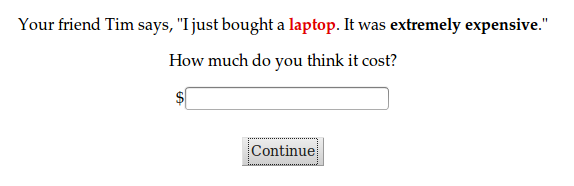
\includegraphics[width=0.45\textwidth]{screenshot.png}
      \end{center}
      \caption{Free response elicititation from Experiment 1.}
      \label{screenshot-figure}
      \end{figure}
      
  \subsubsection{Results}
  
  In a mixed effects linear model of the raw data with fixed effects of surprisal and syllable length and random effects of item and participant, we found no significant effect of either surprisal or syllable length on participants' responses (Figure~\ref{raw-figure}, surprisal: est=616.66, p=0.58; syllable length: est=-213.25, p=0.92).
  
  However, when we z-scored by both participant and item, thereby standardizing different participants beliefs about different items' prices and the ranges of those prices, we do find a significant effect of both surprisal and syllable length (Figure~\ref{scaled-figure}, surprisal: est=0.3336, p$<$2e-16; syllables: est=1.3571, p=1.0e-13).\footnote{We also see a significant negative interaction (est=-0.0949, p=4.8e-12) between the two measures. I'm not sure why this is.}
  
  \begin{figure}[ht]
  \begin{center}
  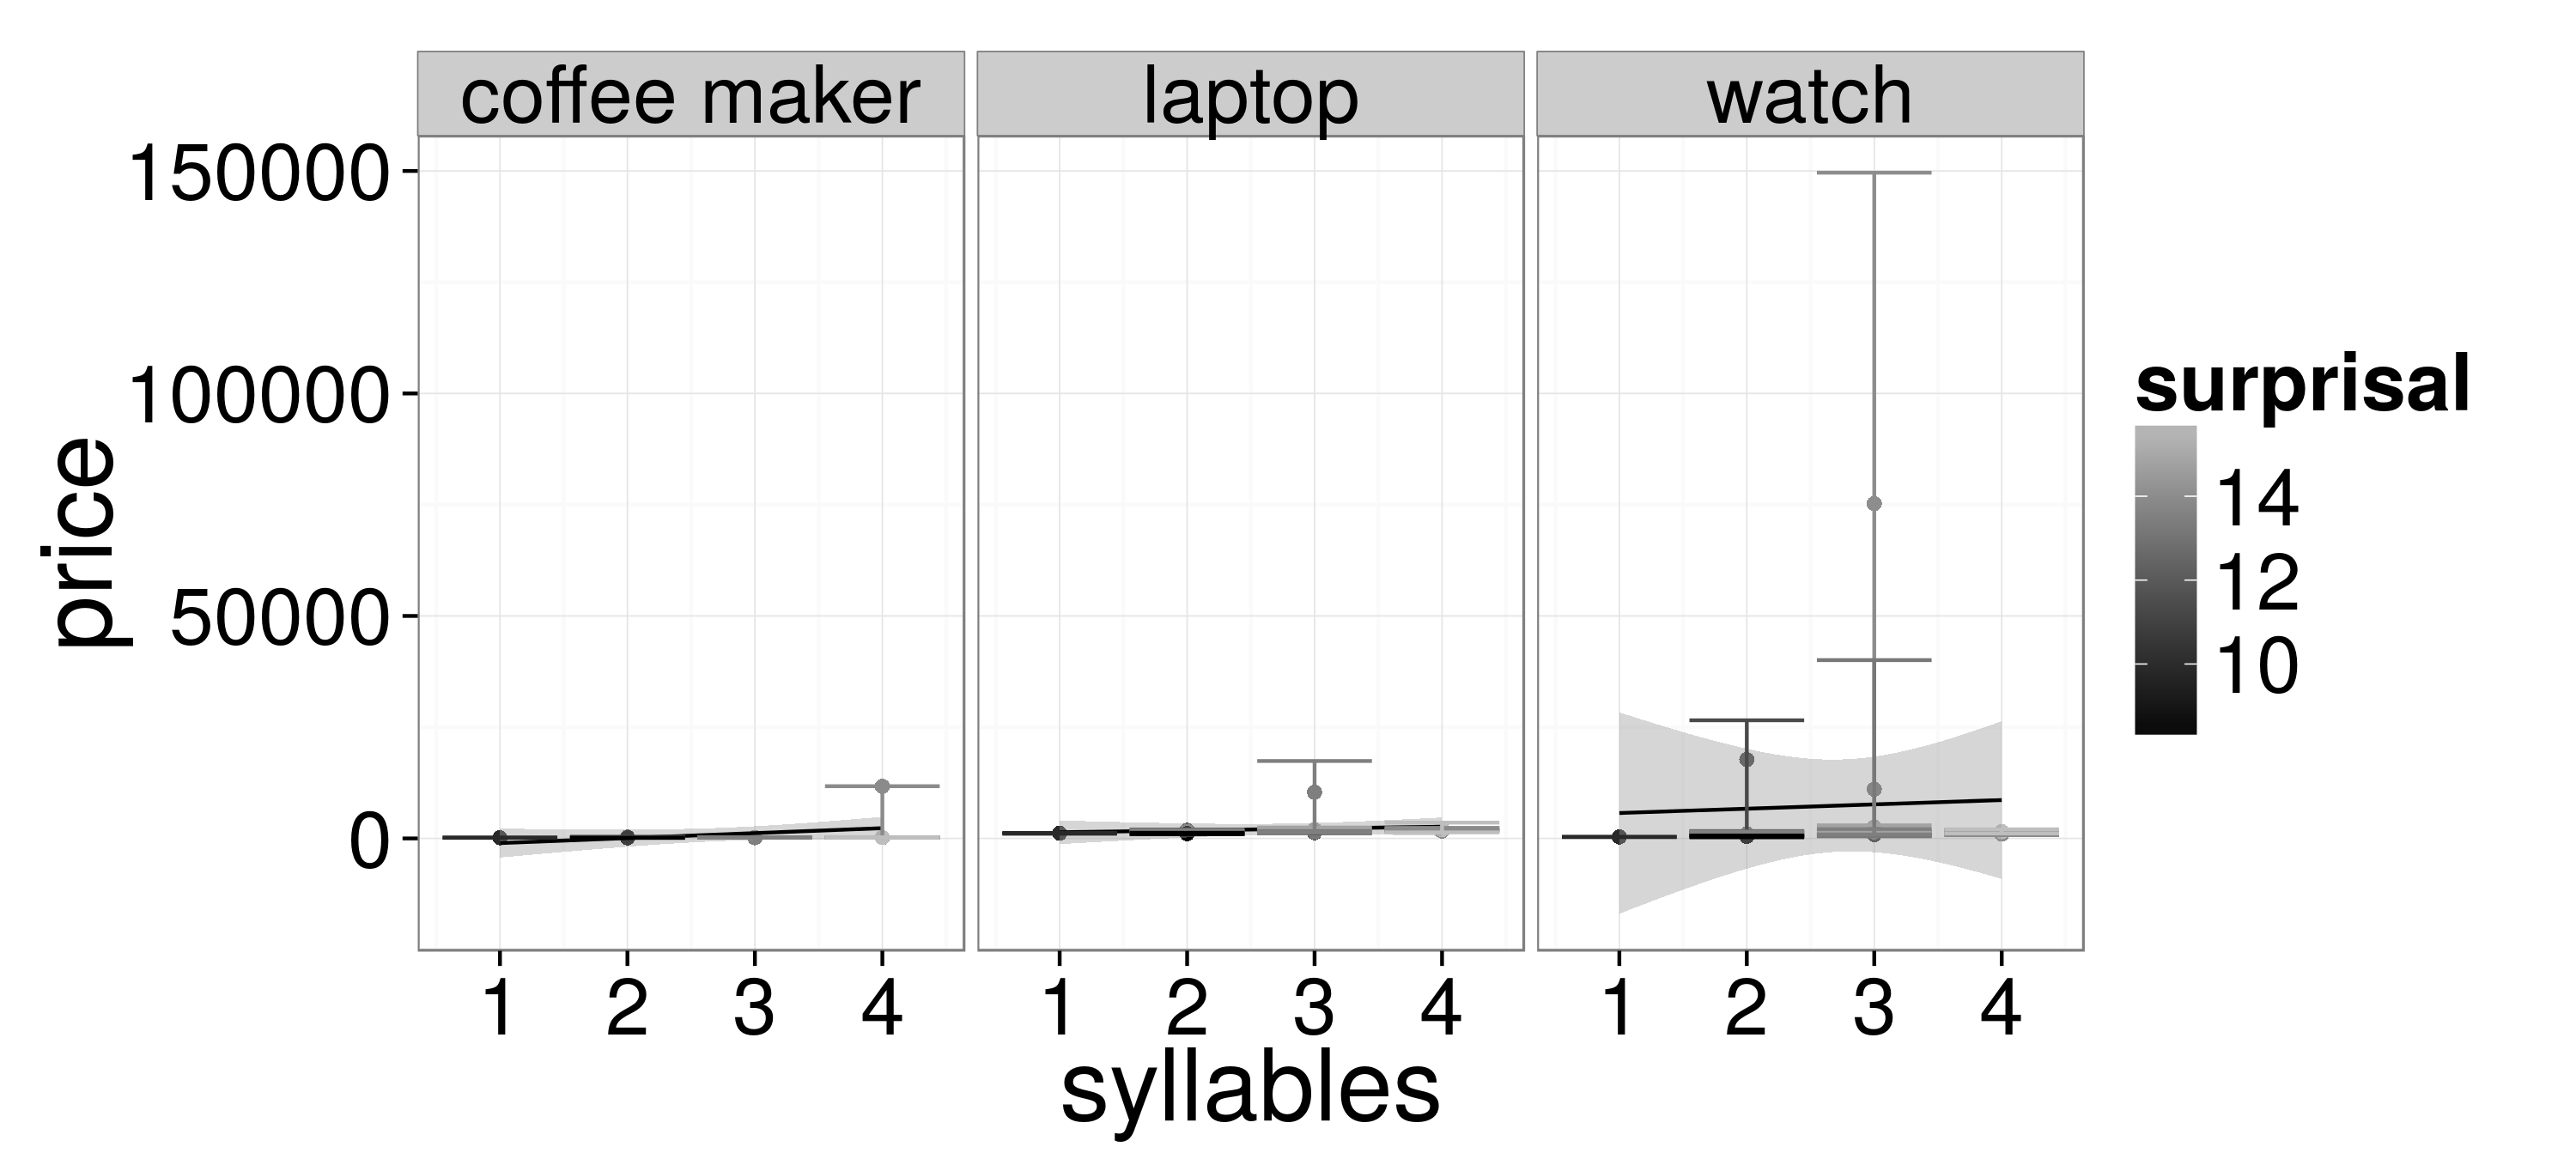
\includegraphics[width=0.45\textwidth]{exp1-raw-syllables.png}
  \end{center}
  \caption{Syllable length versus response in raw data from Experiment 1. Between participants variation in scale, as well as between item differences, make these data difficult to interpret.} 
  \label{raw-figure}
  \end{figure}
  
  \begin{figure}[ht]
  \begin{center}
  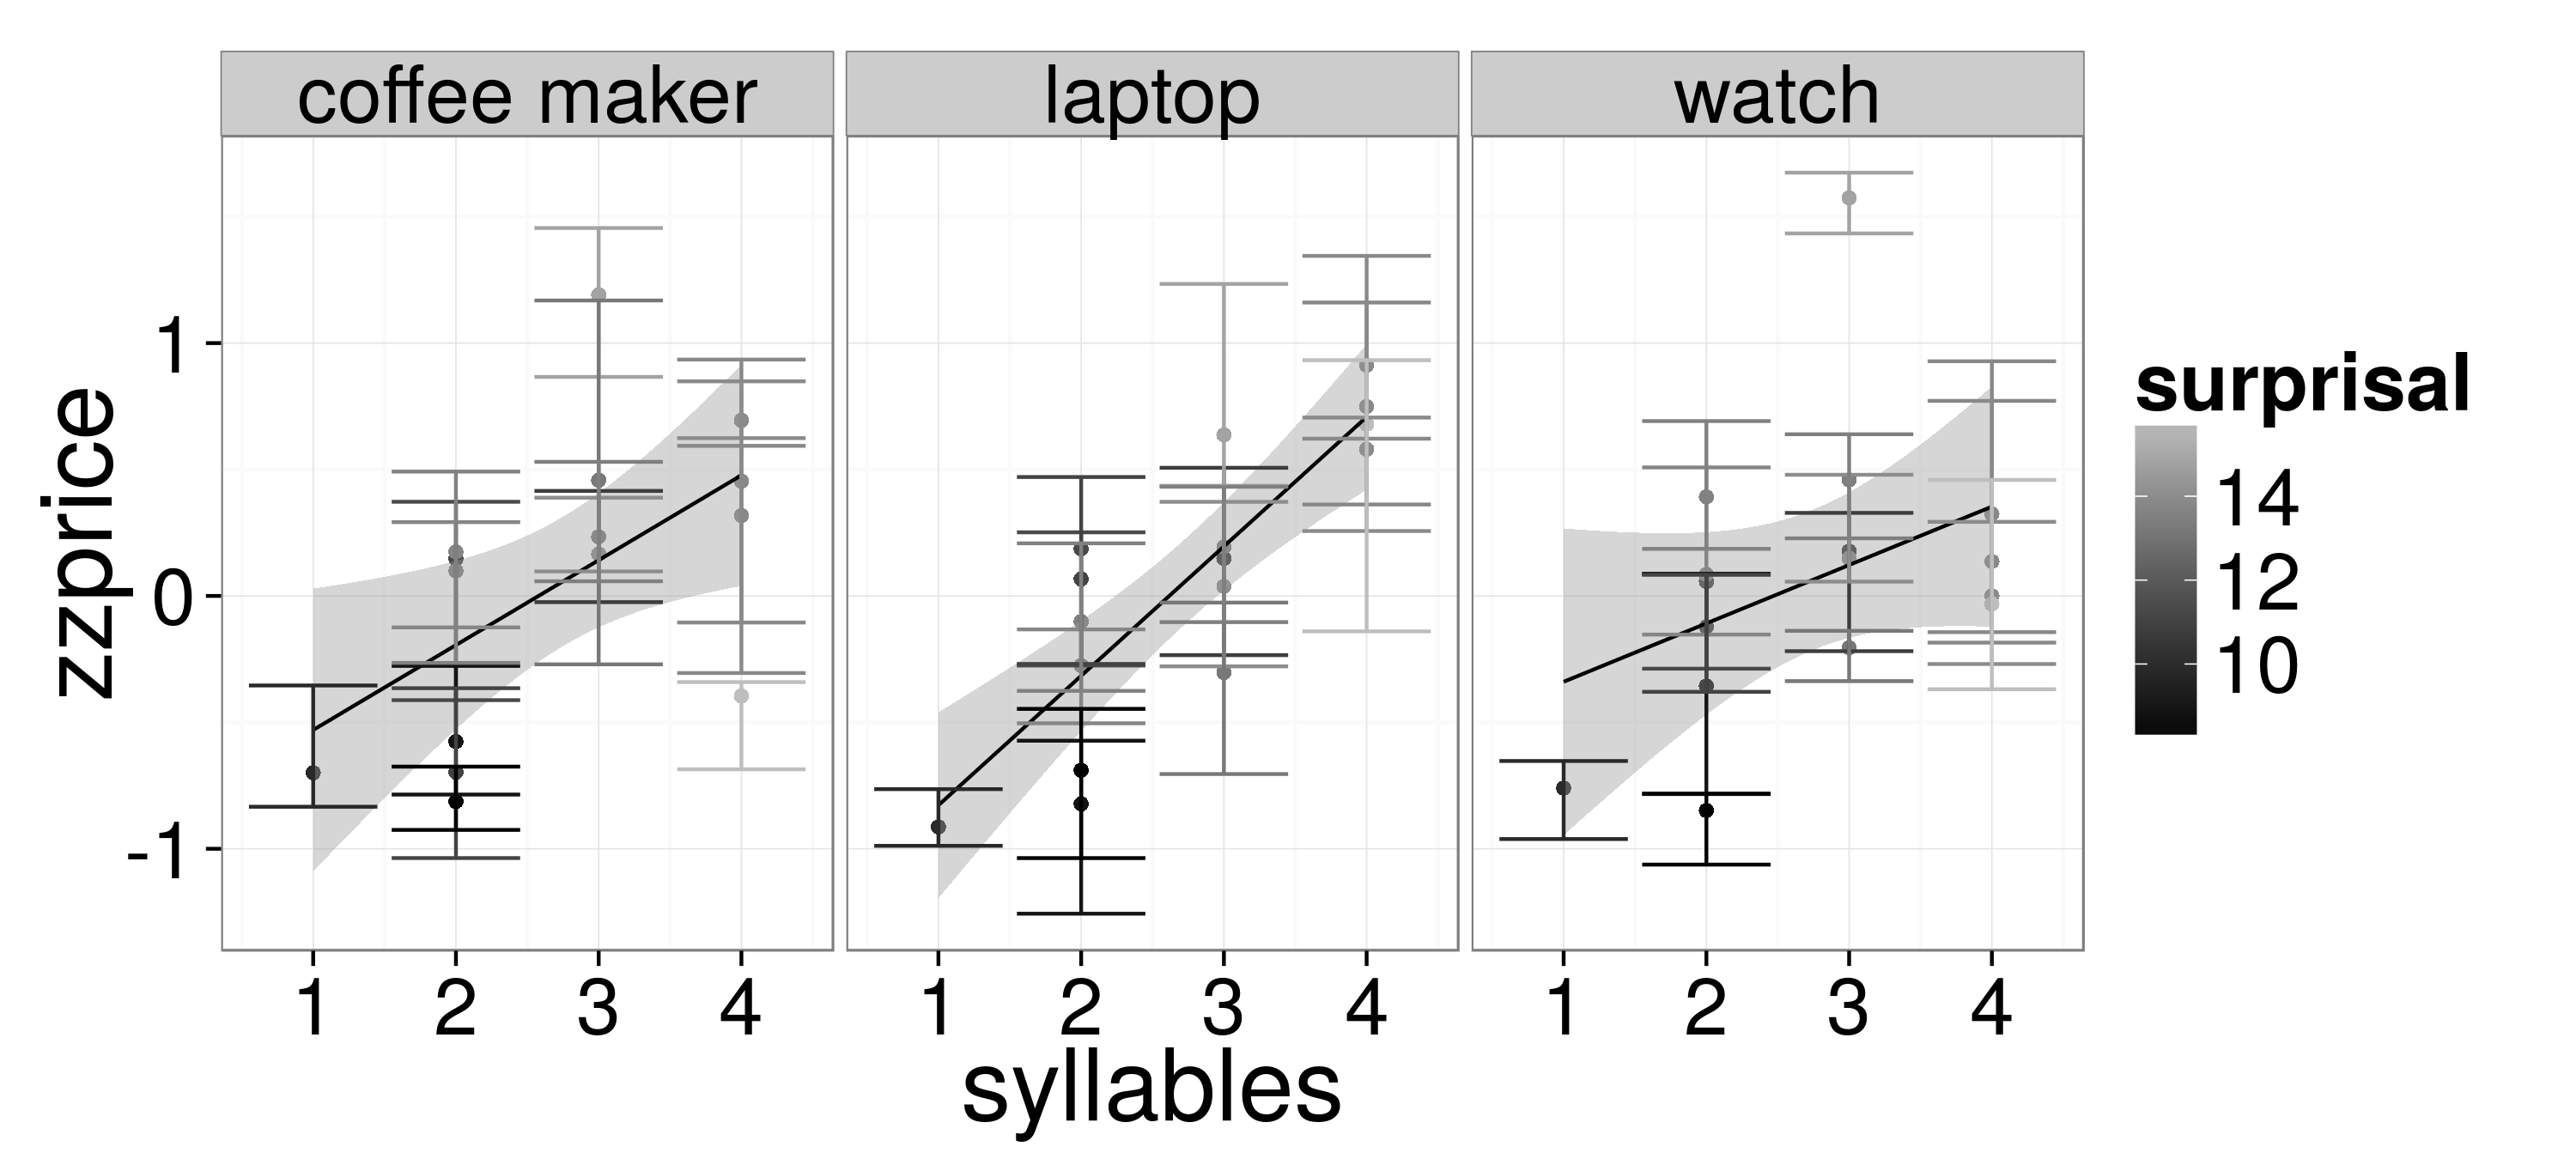
\includegraphics[width=0.45\textwidth]{exp1-zz-syllables.png}
  \end{center}
  \caption{Syllable length versus response in z-scored data from Experiment 1. Responses increase as a function of length in syllables and of surprisal.} 
  \label{scaled-figure}
  \end{figure}
  
  \subsection{Discussion}
  
  Our results provide evidence that cost might be a factor in determining the meaning of a degree adverb. Both syllable length and surprisal predict participants' responses.
  
  One competing explanation for the role of surprisal in Experiment 1 might be that stronger degree adverbs, because they explain things that are more unusual and therefore possibly more rare and less frequently talked about, are consequently said less frequently. That is, perhaps the rarity does not cause the meaning, but rather the meaning causes the rarity. Although this explanation does not account for why syllable length should predict degree adverb strength above and beyond surprisal, we ran Experiment 2 to try to rule out this competing explanation. 
  
\section{Experiment 2: deintensifiers}

  If it were the case that objects that are more extreme along a scale are less common and therefore talked about less, and so the words that describe them (stronger degree intensifying adverbs) are consequently less frequent, then stronger deintensifying adverbs, which describe items more typical along a scale and therefore perhaps more common, would be more frequent in a corpus. Therefore, for deintensifying adverbs, we would again expect a positive relationship between surprisal and price (since all of our items are ``expensive'', the lower the price, the more typical an item would be along the price scale).
  
  If, on the other hand, the meaning of a degree adverb is stronger the less common it is as a result of the additional cost of uttering it, we would expect a negative relationship between surprisal and price for deintensifying adverbs.
  
  We ran Experiment 2 to disentangle these two hypotheses.

  \subsection{Method}
    \subsubsection{Participants}
    We recruited 40 participants on Amazon's Mechanical Turk.
    \subsubsection{Procedure and Materials}
      
      Our procedure was the same as in Experiment 1, except that we drew our degree adverbs from a set of 7 deintensifiers (Table~\ref{deintensifiers-table}) and added the additional item \emph{headphones}.
      
      In addition, since we had degree adverbs of varying word lengths, we used $-log(frequency)$ for each word rather than surprisal. Since these values are proportional to one another, this is sufficient for determining whether a relationship exists between surprisal and responses.
      
      The surprisals and syllable lengths of these degree adverbs were again correlated (0.4903468).
      
      \begin{table}[!ht]
      \begin{center} 
      \caption{Deintensifying degree adverbs from Experiment 2.} 
      \label{deintensifiers-table} 
      \vskip 0.12in
      \begin{tabular}{lrr} 
      \hline
      Deintensifier    &  Frequency & Syllable length \\
      \hline
      kind of & 43691232 & 2 \\ 
      a bit & 33634149 & 2 \\ 
      slightly & 28523541 & 2 \\ 
      sort of & 19227411 & 2 \\ 
      somewhat & 14075405 & 2 \\ 
      moderately & 1922506 & 4 \\ 
      a tad & 775965 & 2 \\  
      \hline
      \end{tabular} 
      \end{center} 
      \end{table}
  \subsubsection{Results}     
    
    We found no evidence for the competing hypothesis (that stronger deintensifying adverbs of degree are more common) (Figure~\ref{exp2-zz}). We also did not find evidence that stronger deintensifying degree adverbs are rarer or longer: in fact, we found a slight positive correlation between syllable length and response (Figure~\ref{exp2-zz-syllables}), implying that longer deintensifying adverbs are less strong. Though since we only have one example of a deintensifying adverb of any syllable length other than 2, this finding should be taken with a grain of salt.
  
    \begin{figure}[ht]
    \begin{center}
    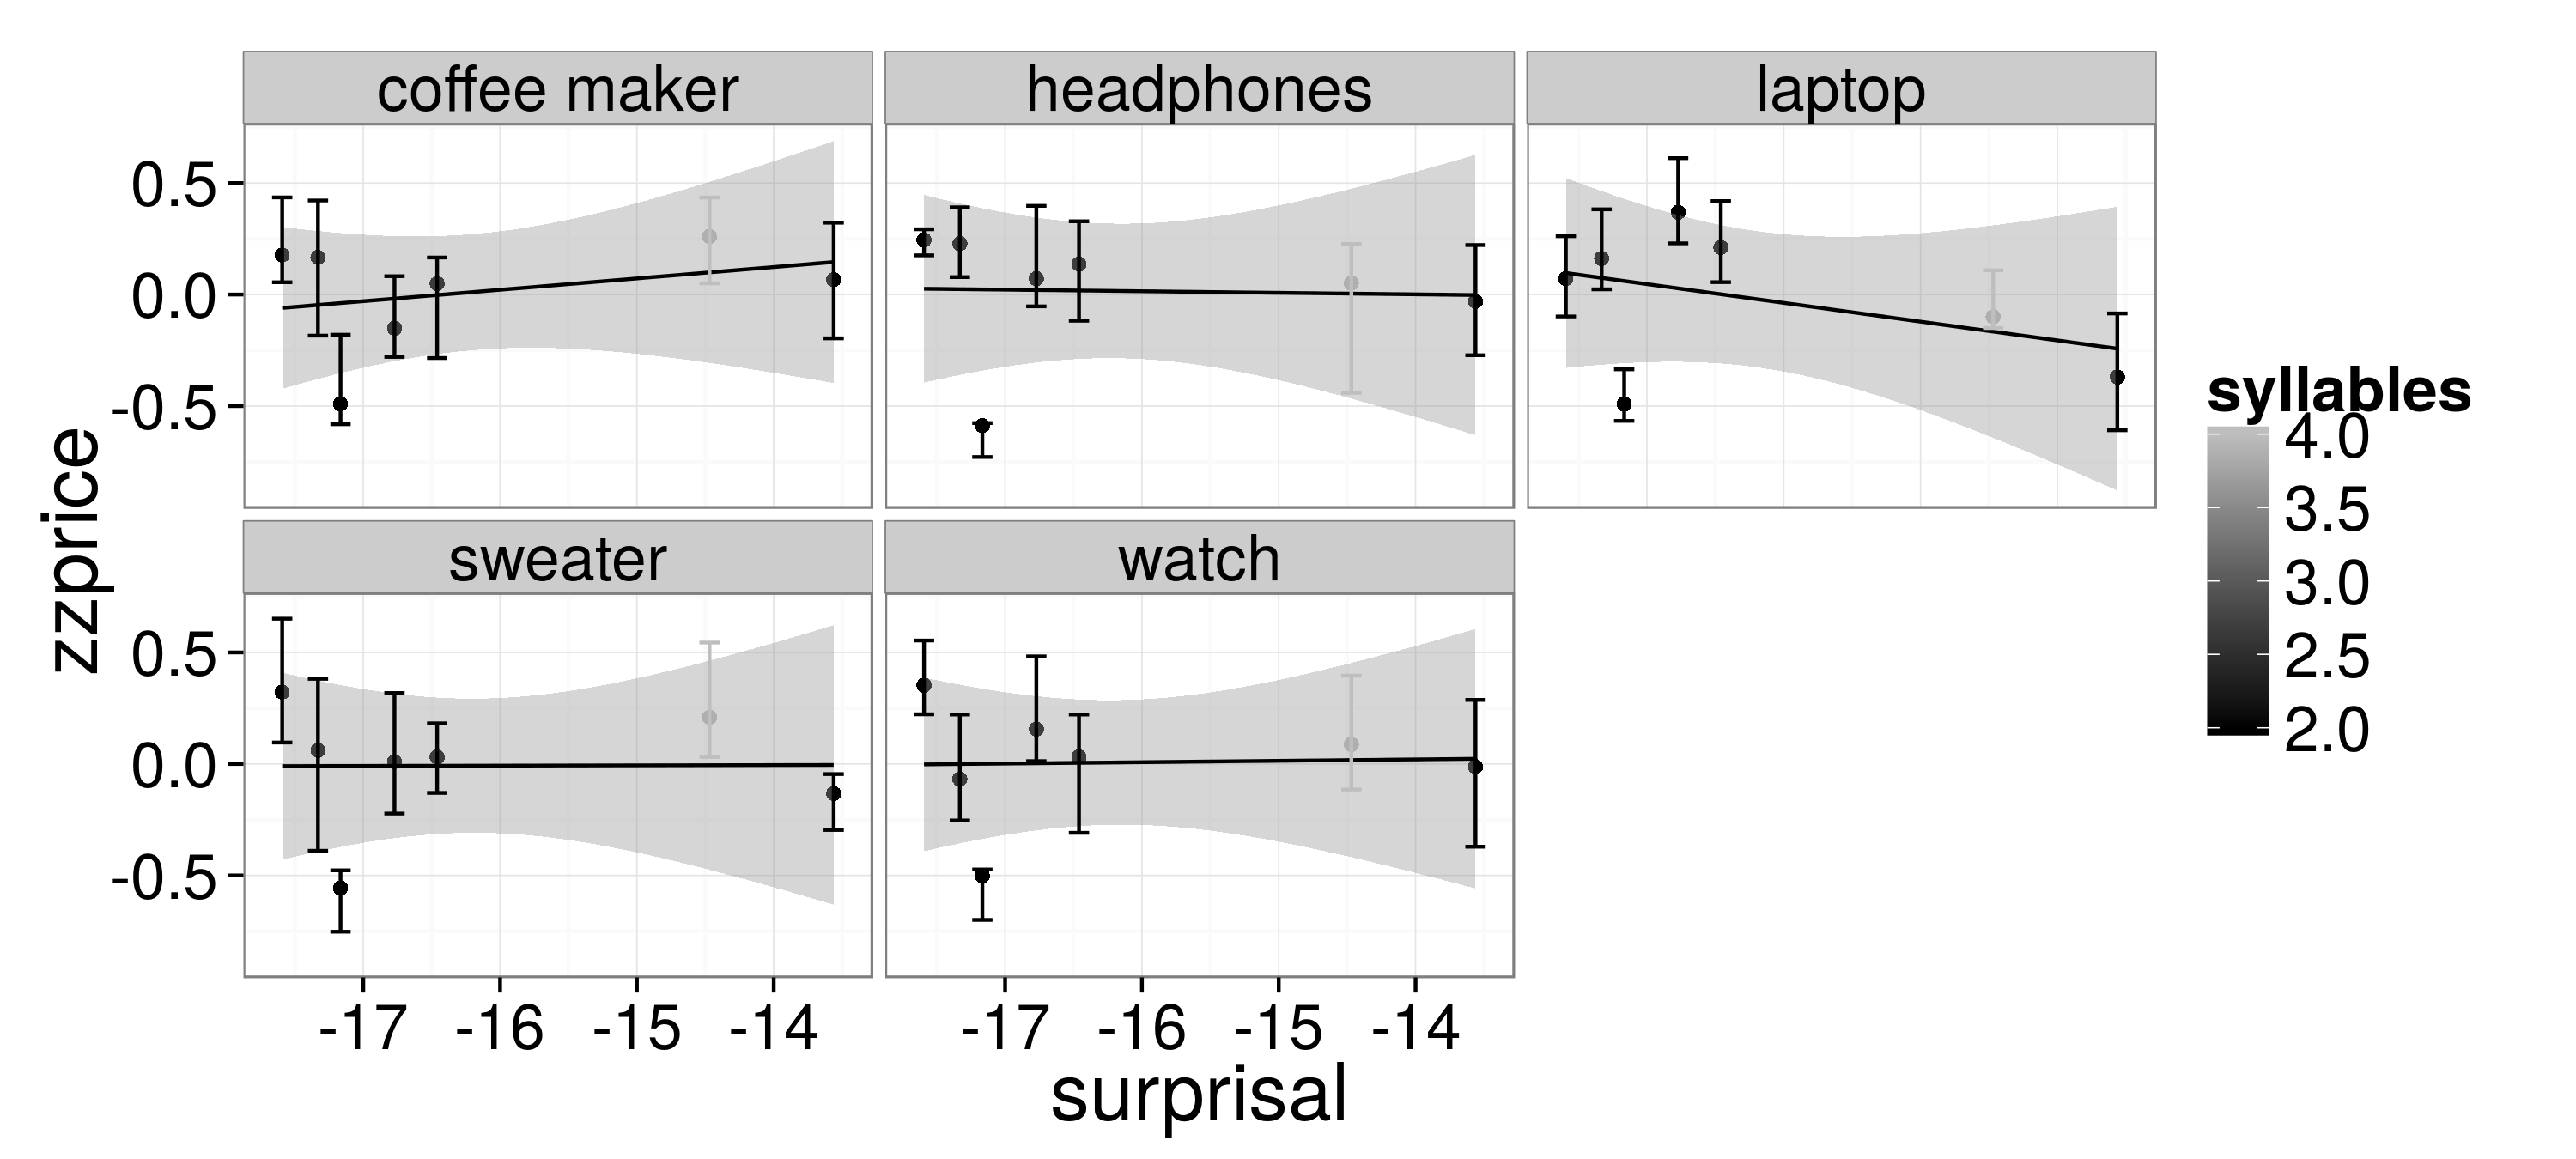
\includegraphics[width=0.45\textwidth]{exp2-zz.png}
    \end{center}
    \caption{Surprisal versus response in z-scored data from Experiment 2.} 
    \label{exp2-zz}
    \end{figure}
    
    \begin{figure}[ht]
    \begin{center}
    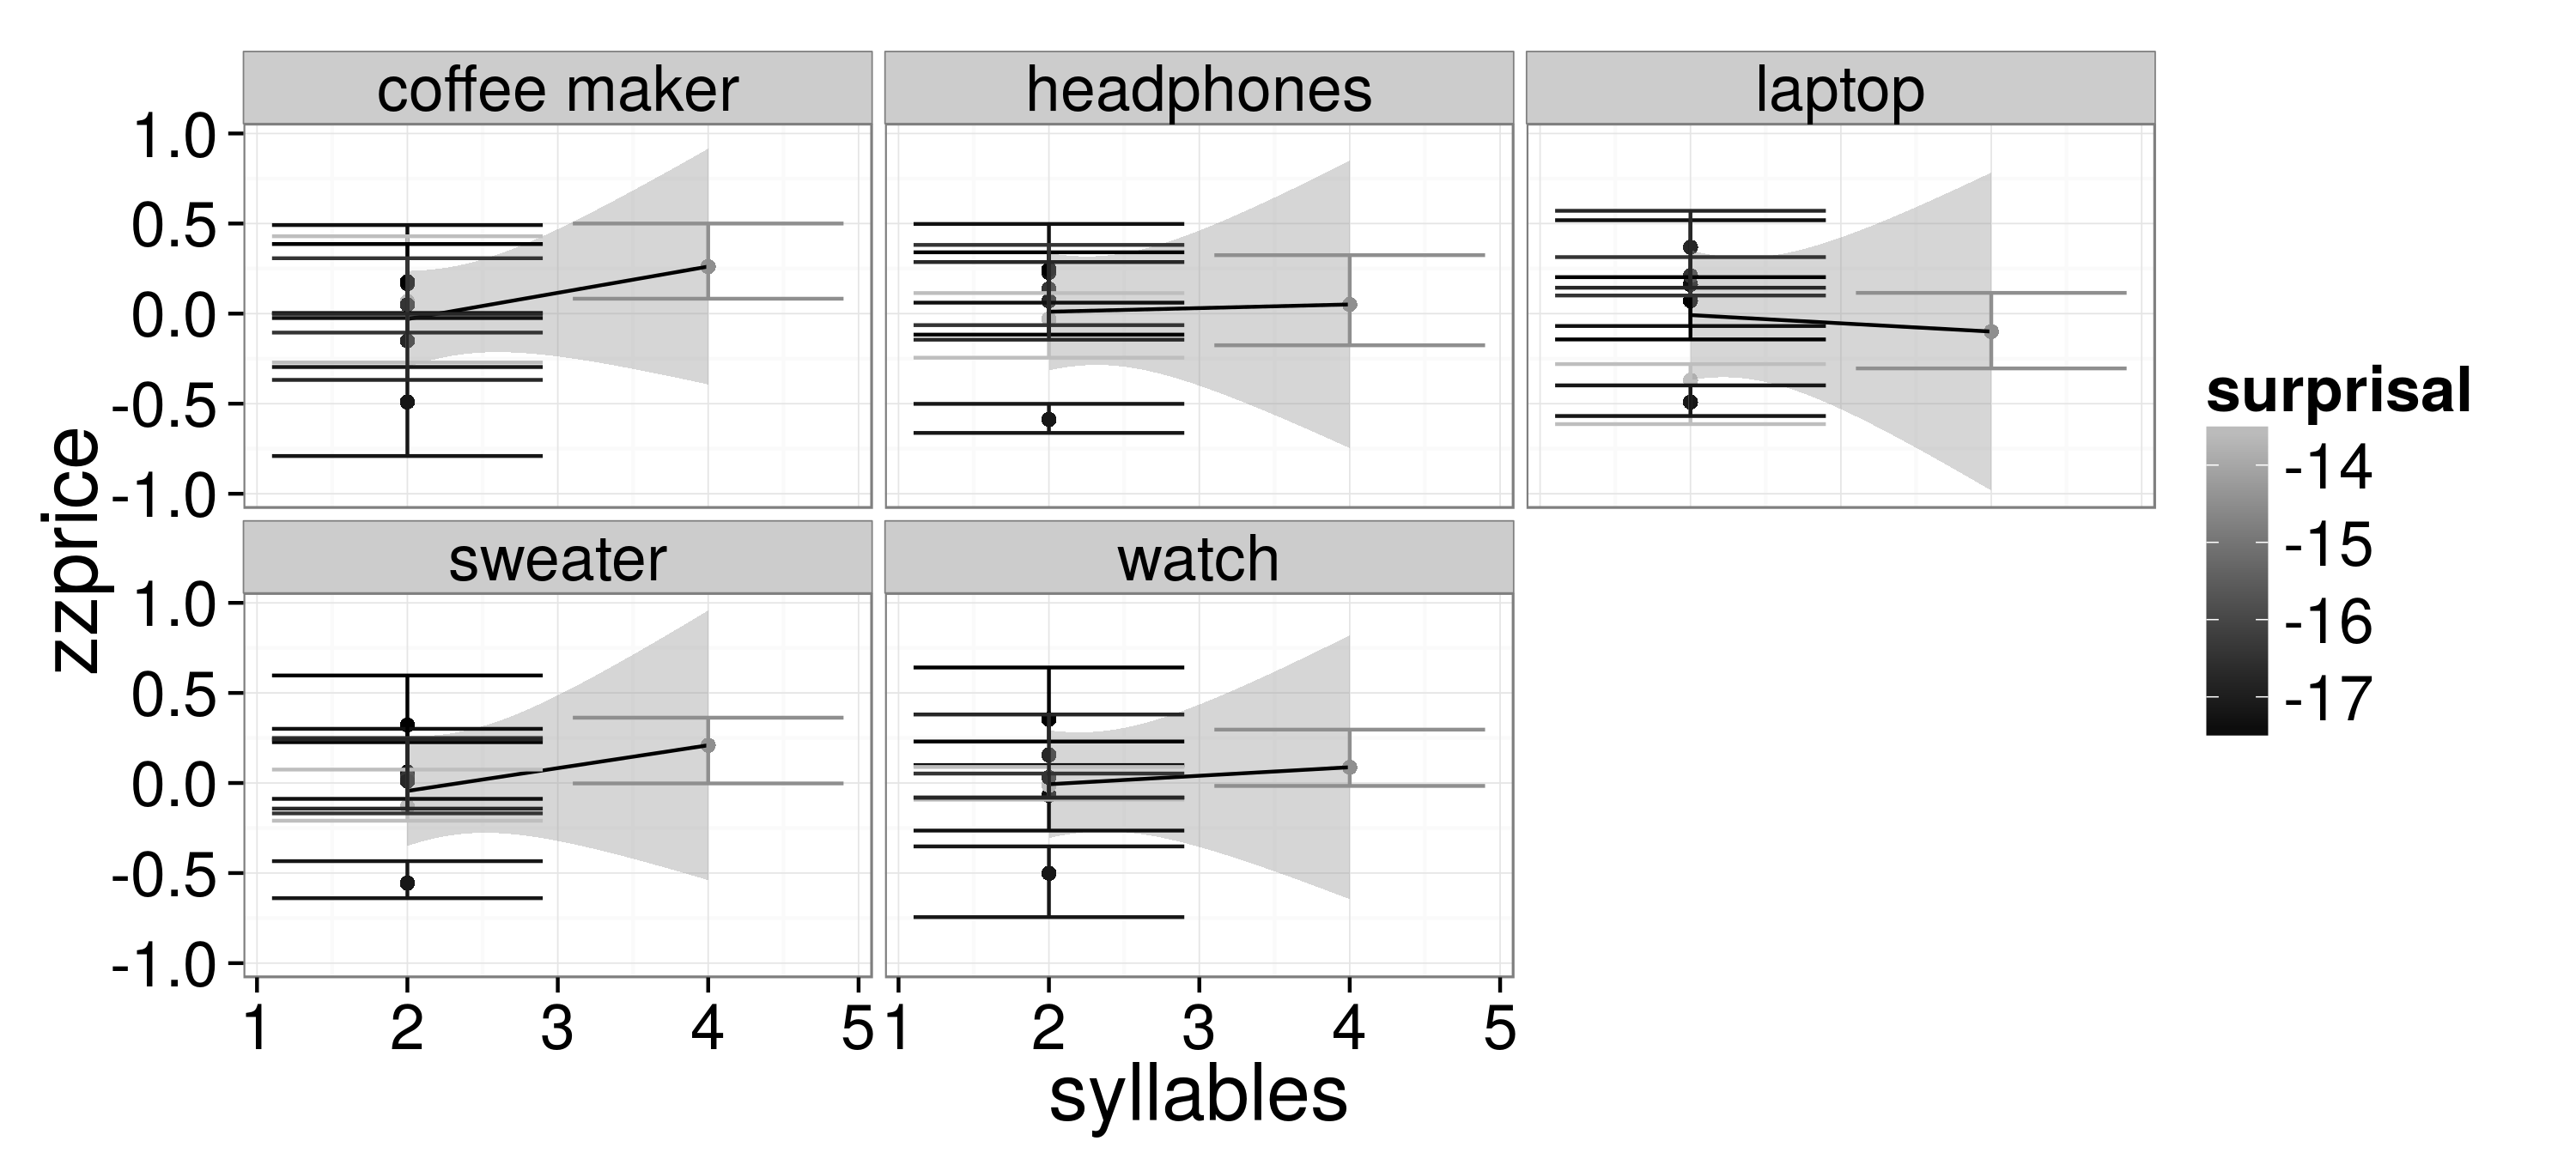
\includegraphics[width=0.45\textwidth]{exp2-zz-syllables.png}
    \end{center}
    \caption{Syllables versus response in z-scored data from Experiment 2.} 
    \label{exp2-zz-syllables}
    \end{figure}
    
  \subsection{Discussion}
  
    Our findings were inconclusive between the two hypotheses, which might indicate that neither is true, that both are true and their effects compete against each other for deintensifiers, or our assumptions about the meanings of deintensifiers are not quite right.

\section{Experiment 3: replication}
  \subsection{Method}
    \subsubsection{Participants}
      We recruited 10 participants on Amazon's Mechanical Turk.
    \subsubsection{Procedure and Materials}
    
      Our procedure was the same as in Experiment 1, but with a slightly different set of degree adverbs that included both intensifers and deintensifiers (Table~\ref{intensifiers-exp3-table}). We elicited participants' responses on only our original 3 items. We again used $-log(frequency)$ for each word rather than surprisal. The surprisals and syllable lengths of these degree adverbs were again correlated (0.5974078).
  
  \subsubsection{Results}
%     In the same rescaling analysis, for intensifiers we found only a marginally significant effect of surprisal in our 10 participants (Figure ~\ref{exp3-intensifiers}, surprisal: estimate=0.07193, p=0.097; syllables: estimate=0.15853,p=0.498), and for deintensifiers we again found no effects (Figure ~\ref{exp3-deintensifiers}).
%   
    \begin{figure}[ht]
    \begin{center}
    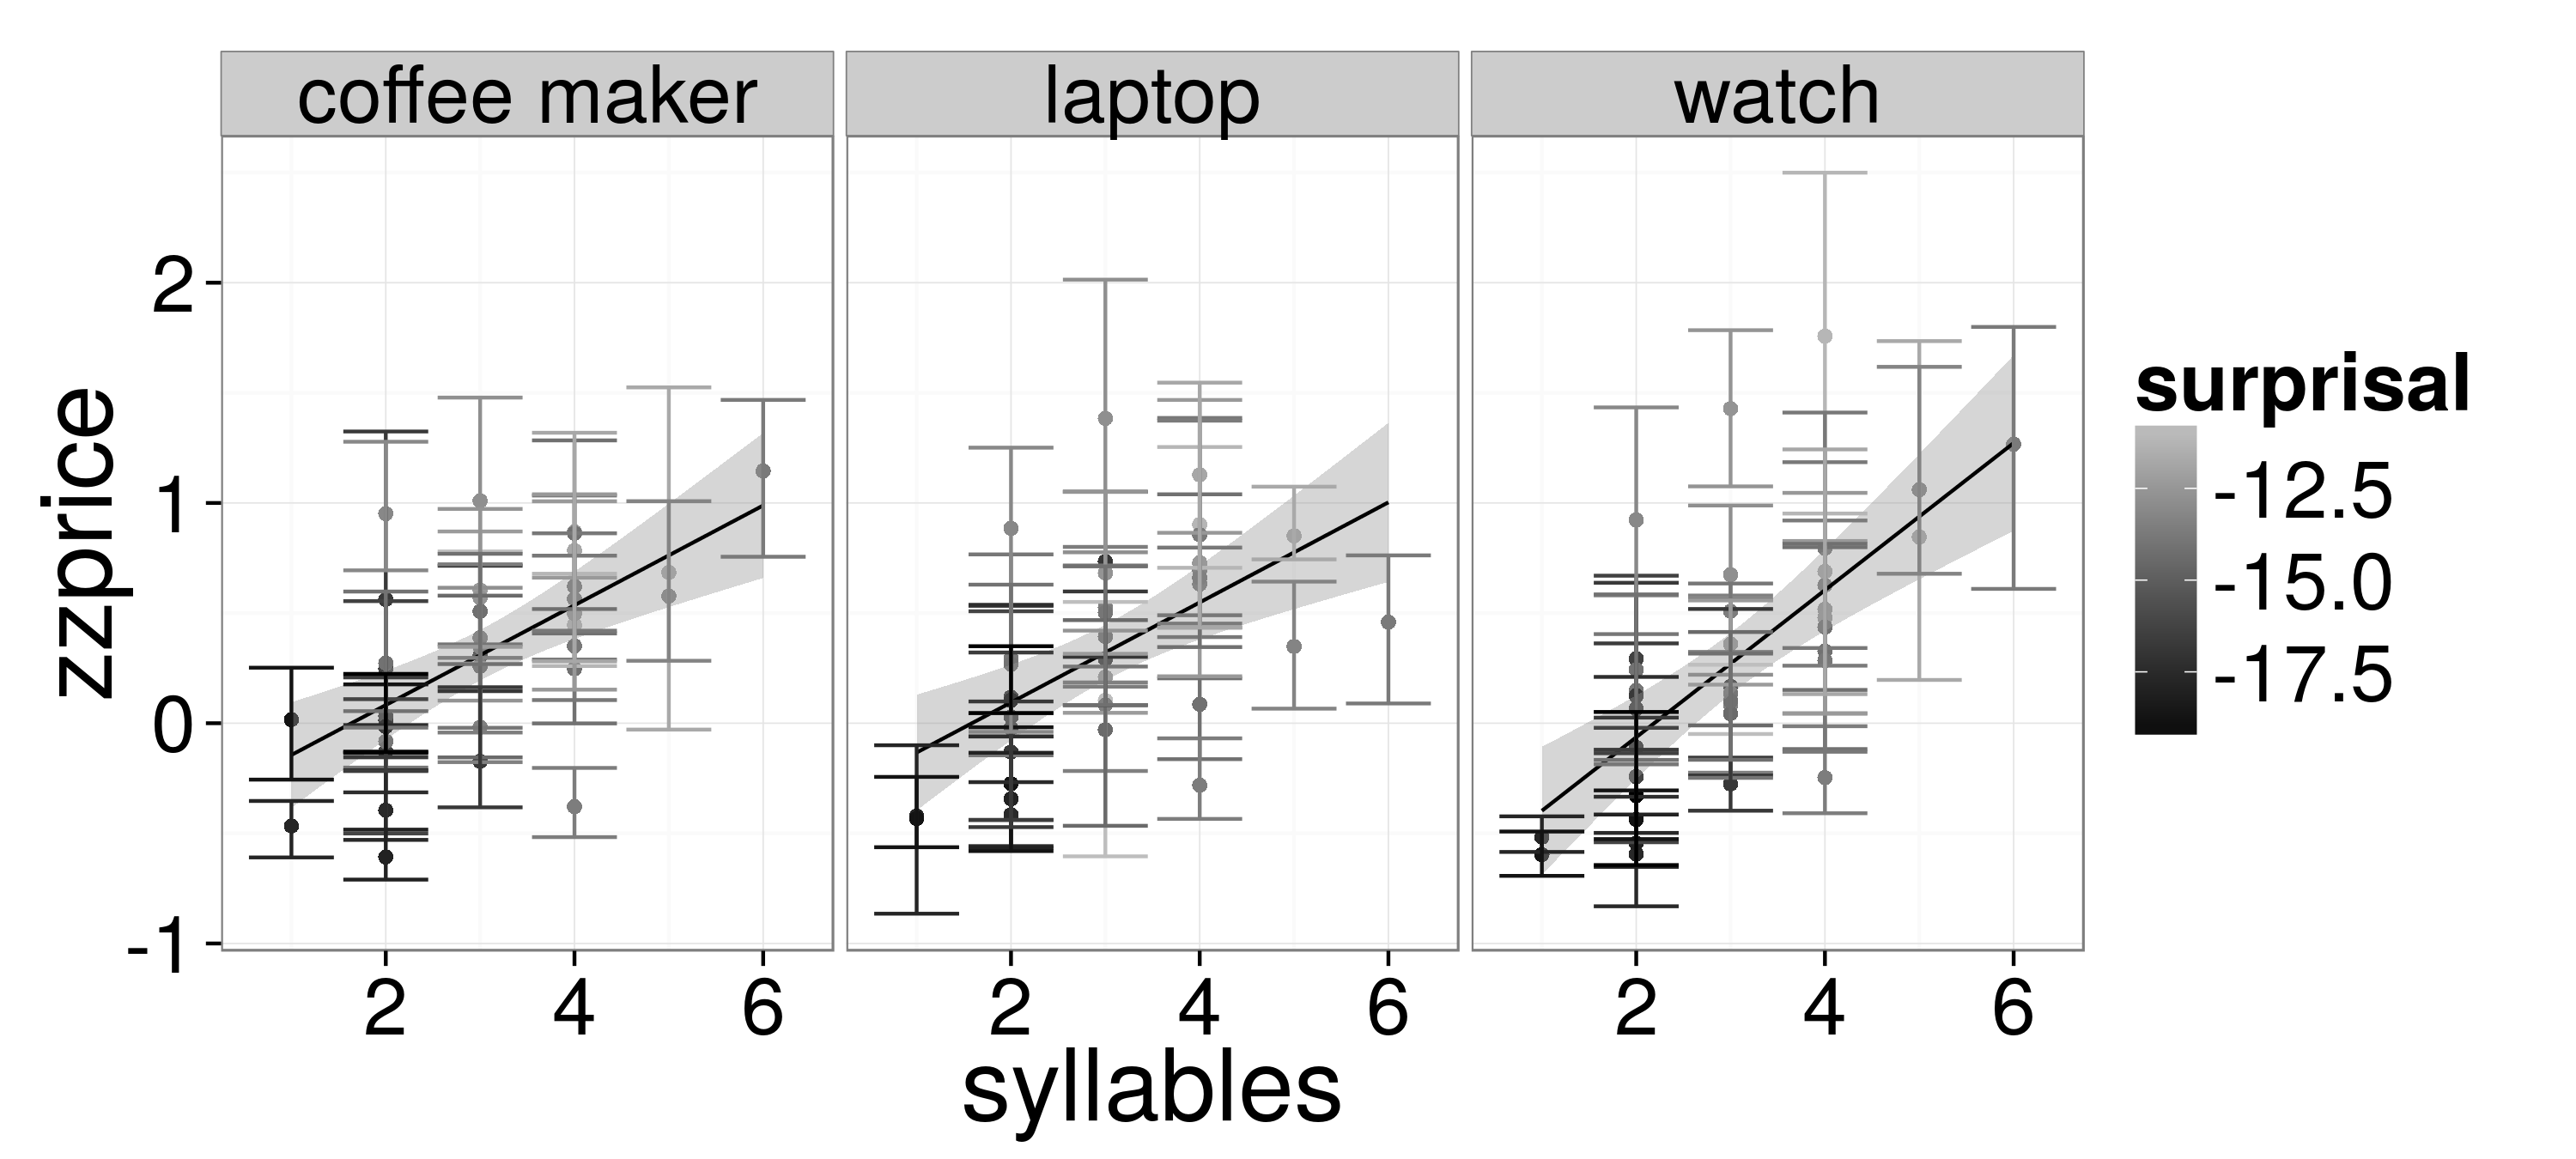
\includegraphics[width=0.45\textwidth]{exp3-intensifiers-zz-syllables.png}
    \end{center}
    \caption{Syllable length versus response in rescaled, augmented data from Experiment 3 (slightly modified replication of Experiment 1).} 
    \label{exp3-intensifiers}
    \end{figure}
    
    \begin{figure}[ht]
    \begin{center}
    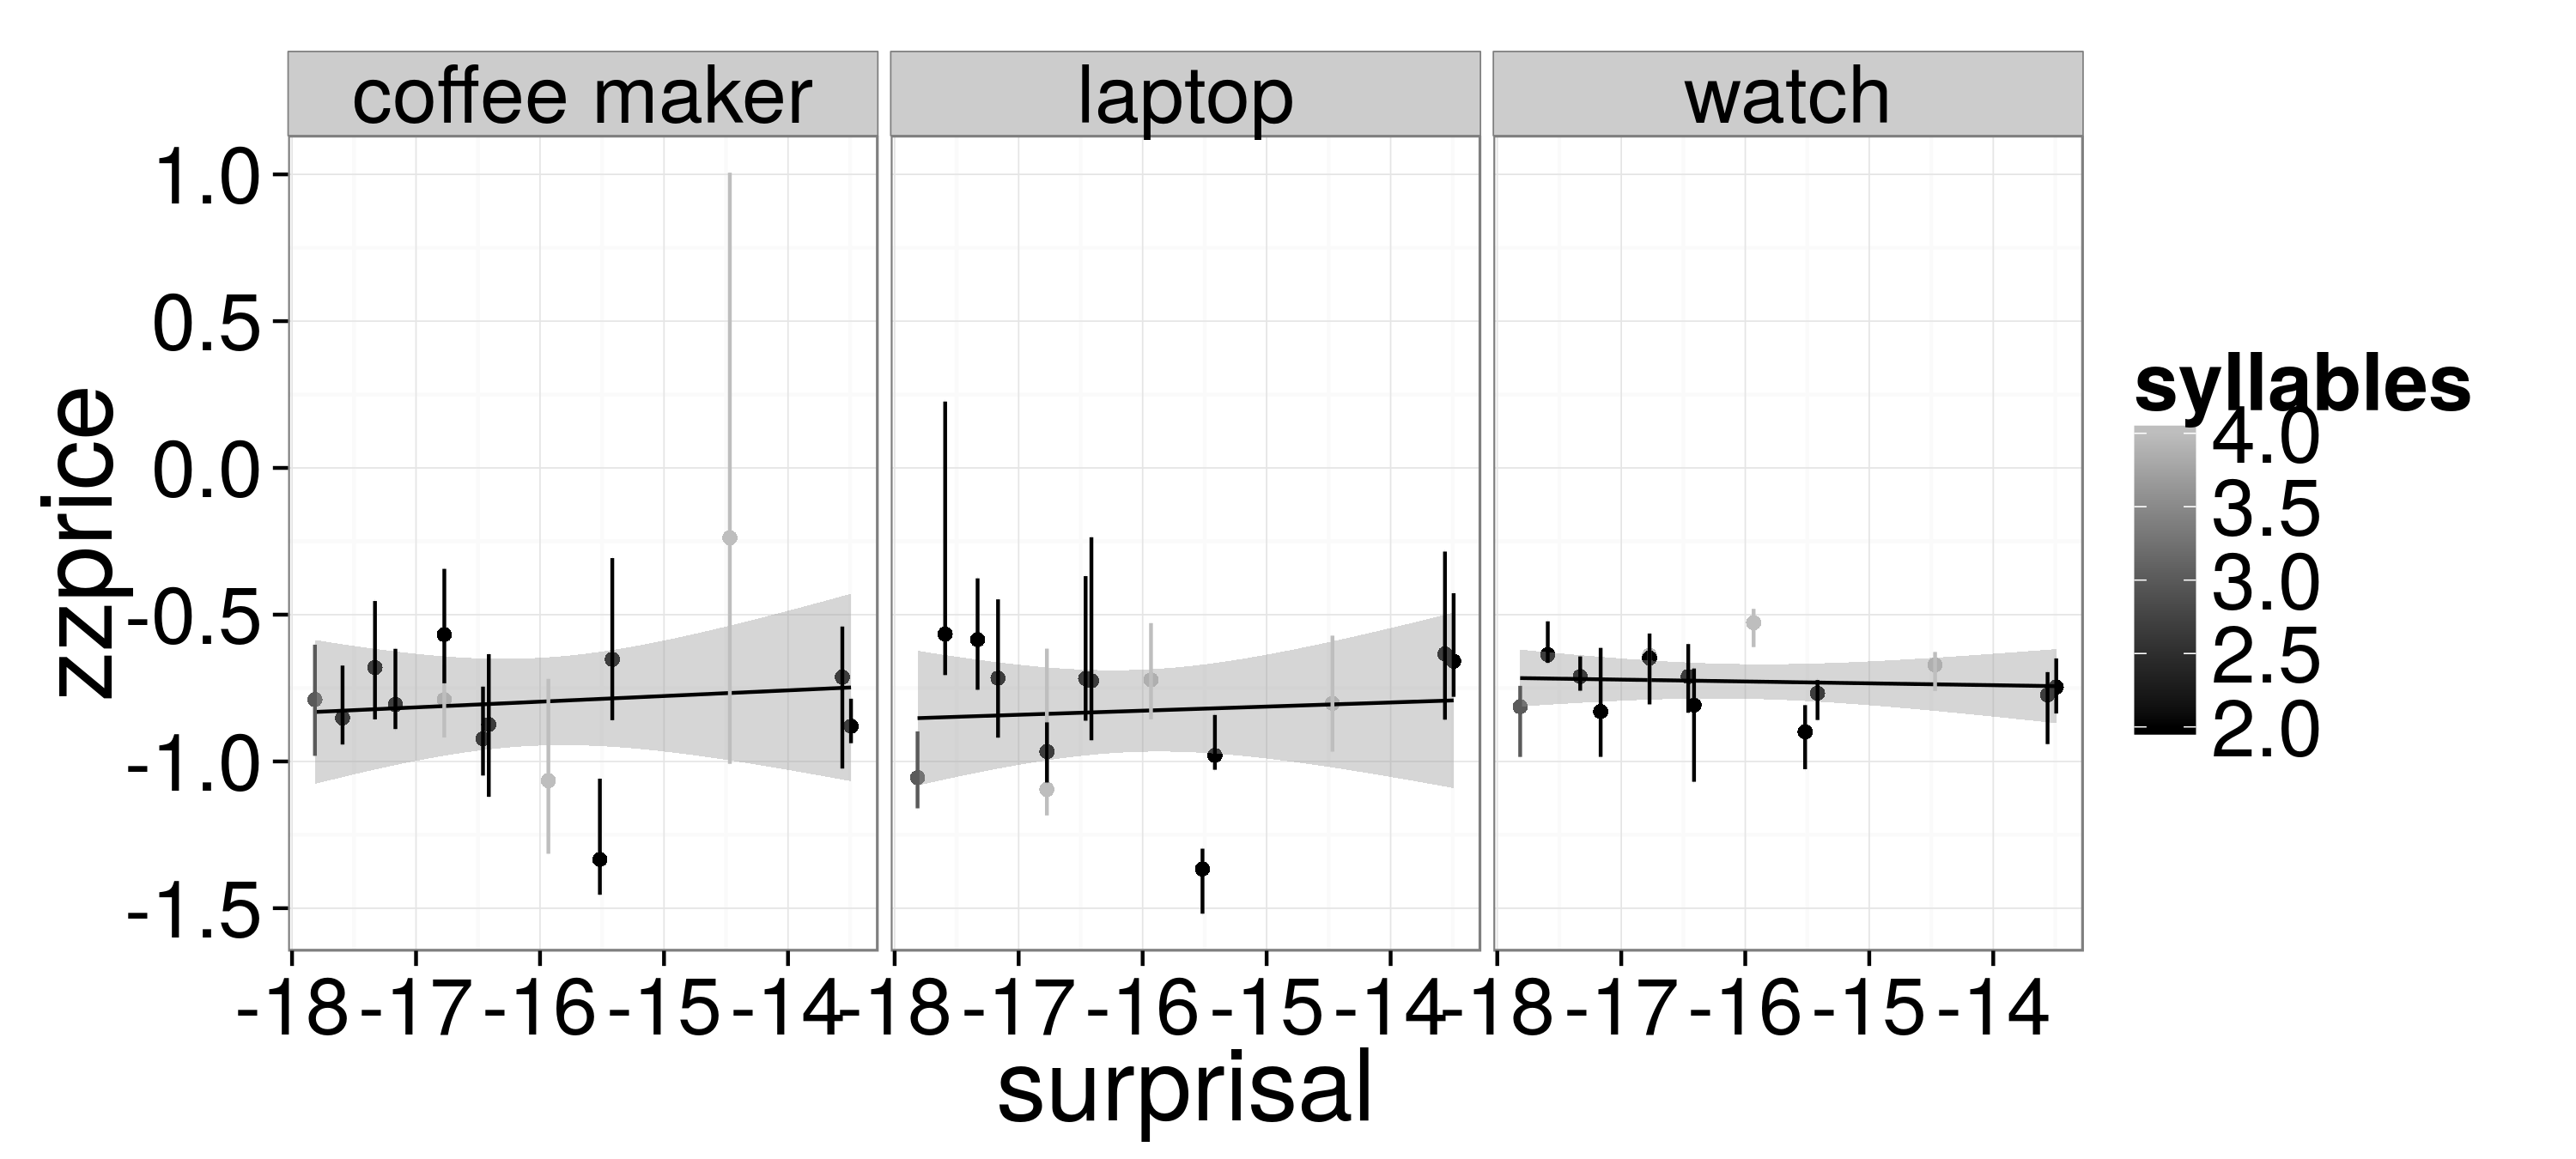
\includegraphics[width=0.45\textwidth]{exp3-deintensifiers-zz.png}
    \end{center}
    \caption{Surprisal versus response in rescaled, augmented data from Experiment 3 (slightly modified replication of Experiment 2)} 
    \label{exp3-deintensifiers}
    \end{figure}
  
  \subsection{Discussion}
  
  We should probably run more participants on this experiment, once we know what the best analysis is.
  
  \section{Conclusion}
  
  We provide some evidence that the strength of a degree adverb might be a function of the cost of that adverb.

% % 
% % \section{Acknowledgments}
% % 
% % Acknowledgments.
% % 
\nocite{web1t5gram}
\nocite{lewis}

\bibliographystyle{apacite}

\setlength{\bibleftmargin}{.125in}
\setlength{\bibindent}{-\bibleftmargin}

\bibliography{degree-adverbs}

      \begin{table}[!ht]
      \begin{center} 
      \caption{Intensifying degree adverbs from Experiment 3.} 
      \label{intensifiers-exp3-table} 
      \vskip 0.12in
      \begin{tabular}{lrr} 
      \hline
      Inntensifier &  Frequency & Syllable length \\
      \hline 
      very        & 292897993 & 2 \\
      really      & 148918637 & 2 \\ 
      real        & 144660526 & 1 \\ 
      rather      &  66341863 & 2 \\ 
      quite       &  55269390 & 1 \\ 
      pretty      &  43623658 & 2 \\ 
      highly      &  36460329 & 2 \\ 
      slightly    &  28523541 & 2 \\ 
      extremely   &  21862963 & 3 \\ 
      totally     &  20950052 & 3 \\ 
      truly       &  19778608 & 2 \\ 
      super       &  16902202 & 2 \\ 
      crazy       &  13048828 & 2 \\ 
      greatly     &  11337773 & 2 \\ 
      terribly    &   1906059 & 3 \\ 
      wildly      &   1414395 & 3 \\ 
      radically   &   1414254 & 4 \\ 
      amazingly   &   1384225 & 4 \\ 
      vastly      &   1311113 & 2 \\ 
      intensely   &   1084765 & 3 \\ 
      hugely      &   1074430 & 2 \\ 
      enormously  &   1011751 & 4 \\ 
      exceedingly &    977435 & 4 \\ 
      extraordinarily & 900456 & 6 \\ 
      excessively & 877280 & 4 \\ 
      horribly & 819111 & 3 \\ 
      decidedly & 817806 & 4 \\ 
      ever so & 697737 & 3 \\ 
      ridiculously & 581660 & 5 \\ 
      uber & 503592 & 2 \\ 
      insanely & 359644 & 3 \\ 
      supremely & 296134 & 3 \\ 
      fantastically & 250989 & 4 \\ 
      outrageously & 240010 & 4 \\ 
      stupidly & 224107 & 3 \\ 
      uncommonly & 135747 & 4 \\ 
      phenomenally & 120769 & 5 \\ 
      astoundingly & 73041 & 4 \\ 
      crazily & 52356 & 3 \\
      \hline
      \end{tabular} 
      \end{center} 
      \end{table}
      
      \begin{table}[!ht]
      \begin{center} 
      \caption{Dentensifying degree adverbs from Experiment 3.} 
      \label{deintensifiers-exp3-table} 
      \vskip 0.12in
      \begin{tabular}{lrr} 
      \hline
      Inntensifier &  Frequency & Syllable length \\
      \hline
      a little & 54587448 & 3 \\ 
      kind of & 43691232 & 2 \\ 
      a bit & 33634149 & 2 \\ 
      relatively & 19236549 & 4 \\ 
      sort of & 19227411 & 2 \\ 
      somewhat & 14075405 & 2 \\ 
      fairly & 13432053 & 2 \\ 
      reasonably & 8307027 & 4 \\ 
      barely & 5483661 & 2 \\ 
      kinda & 4961342 & 2 \\ 
      moderately & 1922506 & 4 \\ 
      a tad & 775965 & 2 \\ 
      sorta & 723566 & 2 \\ 
      \hline
      \end{tabular} 
      \end{center} 
      \end{table}

      %mildly is a good deintensifying adverb

\end{document}
